\documentclass[border=2pt]{standalone}

%Drawing
\usepackage{tikz}
\tikzset{>=latex}
\usetikzlibrary{calc, decorations.markings}

%Styles
%%Arrow in the Middle
\tikzset{arrow inside/.style = {postaction=decorate,decoration={markings,mark=at position 0.52 with \arrow{stealth}}}}

%Newcommand
%%Midline Label
\newcommand{\midlinelabel}[3]{
   \node (midlabel) at ($ (#1)!.5!(#2) $) {#3};
   \draw[<-] (#1) --  (midlabel);
   \draw[->] (midlabel) -- (#2);
}

% Define Color
\definecolor{glass}{cmyk}{0.2,0,0,0}

\begin{document}
	
	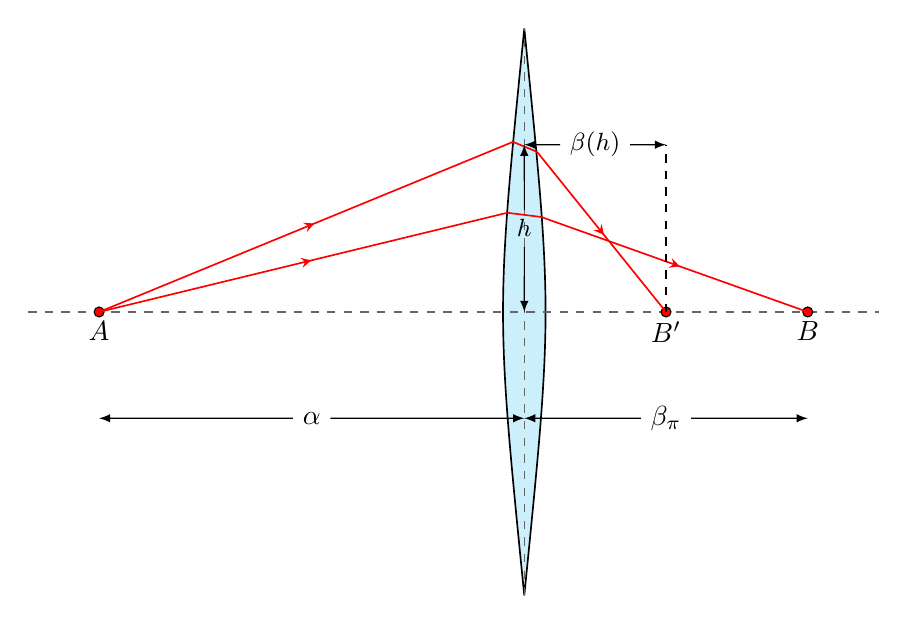
\begin{tikzpicture}[scale=1.8]
		% Grid
%		\draw[help lines] (-3,-3) grid (6,6);
		
		% Lens
		\path[fill=glass, draw=black, line width = 0.6] (1,-2) .. controls (0.8,0) .. (1,2) .. controls (1.2,0) .. (1,-2);
		
		% Axis
		\draw[dashed, black!60] (1,-2) -- +(0,4);
		\draw[dashed, black!60] (-2.5,0) -- (3.5,0);
		
		% Points
		\draw[fill=red] (-2,0) circle (1pt) node[below] {$A$};
		\draw[fill=red] (3,0) circle (1pt) node[below] {$B$};
		\draw[fill=red] (2,0) circle (1pt) node[below] {$B'$};
				
		%Rays
		%%1
		\draw[red, line width = 0.6, arrow inside] (-2,0) -- (0.88,0.7);	
		\draw[red, line width = 0.6] (0.88,0.7) -- (1.12,0.67);
		\draw[red, line width = 0.6, arrow inside] (1.12,0.67) -- (3.,0);
		%%2
		\draw[red, line width = 0.6, arrow inside] (-2,0) -- (0.92,1.2);	
		\draw[red, line width = 0.6] (0.92,1.2) -- (1.09,1.13);
		\draw[red, line width = 0.6, arrow inside] (1.09,1.13) -- (2,0);

		% Distances
		\midlinelabel{-2,-0.75}{1,-0.75}{$\alpha$}
		\midlinelabel{1,-0.75}{3,-0.75}{$\beta_\pi$}
		\midlinelabel{1,0}{1,1.18}{\small$h$}	
		\midlinelabel{1,1.18}{2,1.18}{\small$\beta(h)$}
		
		% Dashed
		\draw[dashed] (2,0) -- (2,1.18);
	\end{tikzpicture}
	
\end{document}